\chapter{Аналитический раздел}
\label{cha:analysis}

Облака - очень сложная и выразительная часть неба. Именно облака могут создать впечатление
о надвигающихся погодных условиях.
Для создания реалистичного неба облака должны визуализироваться в реальном времени.
Есть множество алгоритмов для достижения этой цели.

\section{Анализ предметной области}

\subsection{Методы создания облаков}

Существует три основных метода визуализации облаков. Классический метод подразумевает использование единой панорамной текстуры,
которую необходимо наложить на небесную сферу \cite{Gue14}. Чтобы создать движение в небе, используется техника визуального
потока, при котором панорамная текстура вращается, создавая иллюзию движения облаков в определенном направлении, например,
ветра (рисунок \ref{img:cloud_sphere}). Данный метод является эффективным, однако не позволяет изменять форму облаков, погоду или освещение
(рисунок \ref{img:result_sphere}).

\begin{figure}[H]
    \centering
    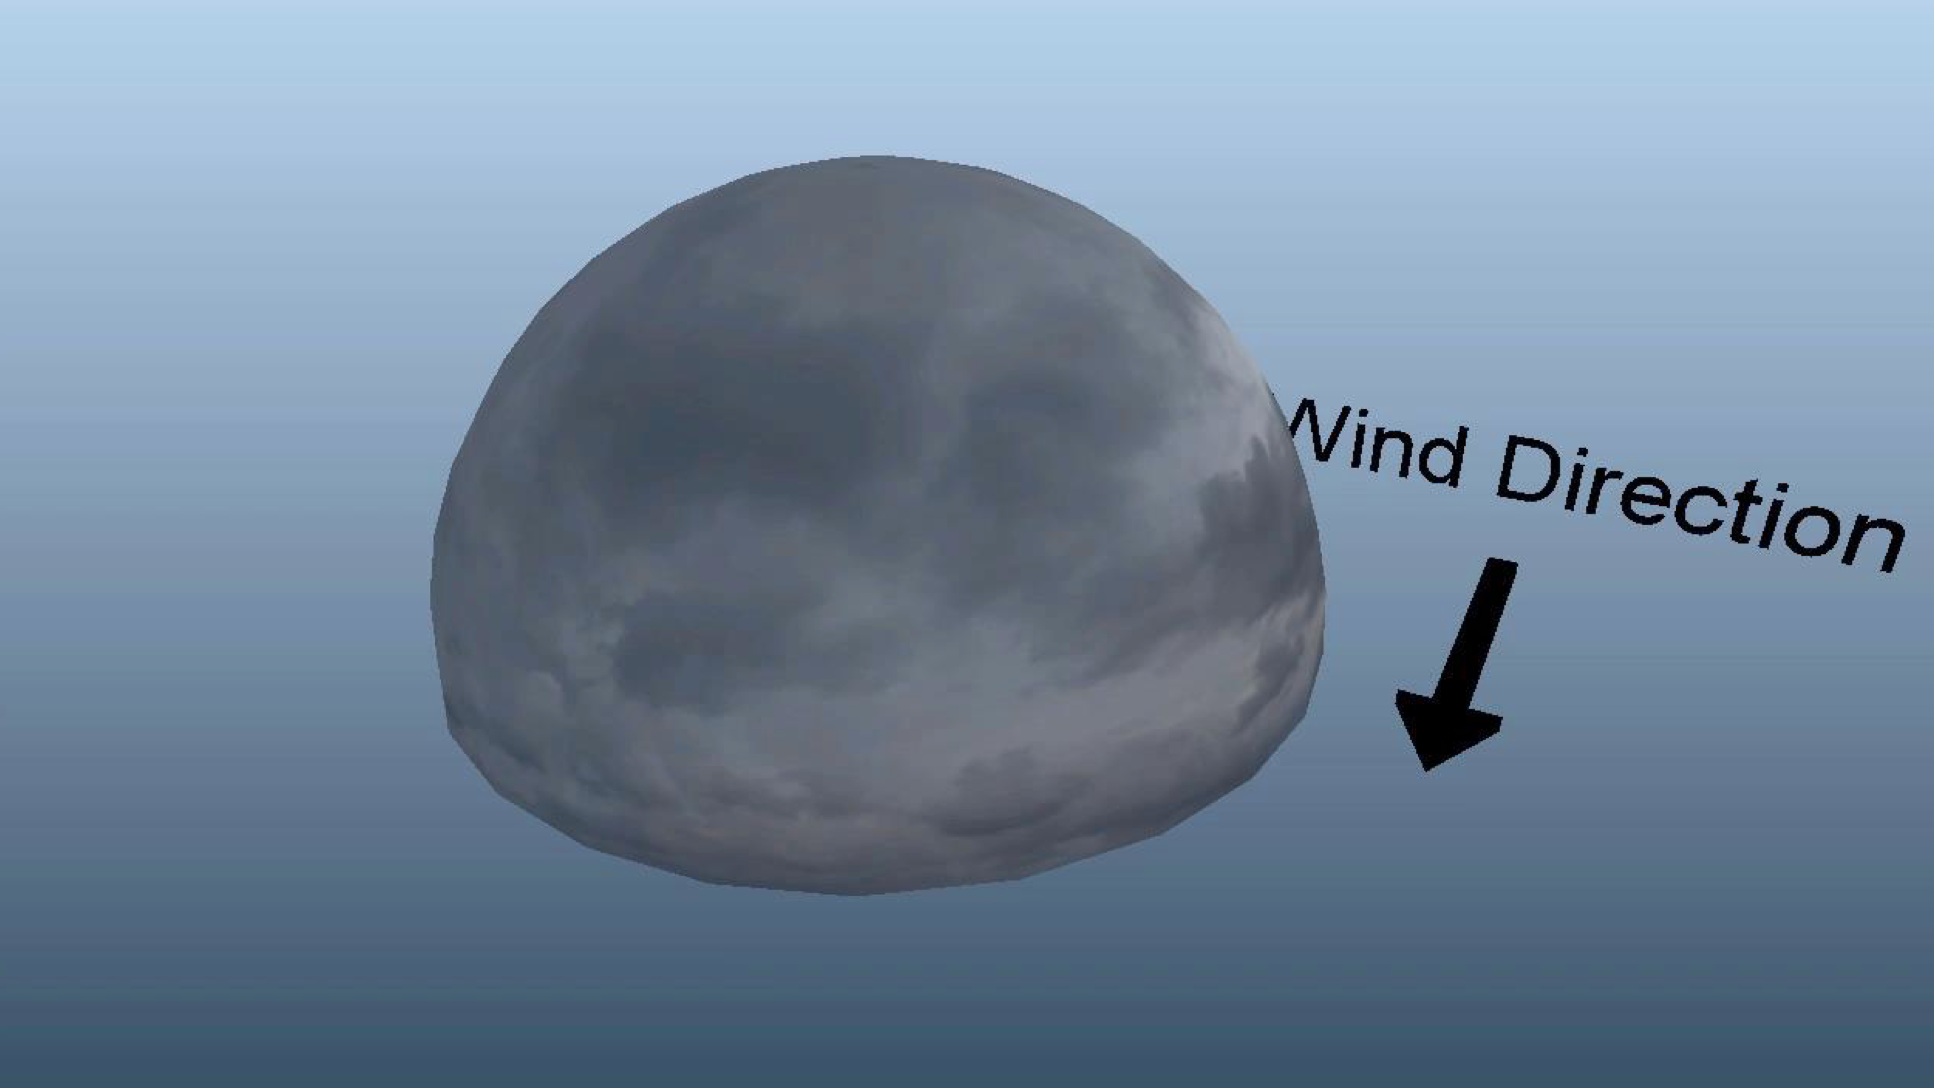
\includegraphics[scale=0.4]{img/cloud_sphere.png}
    \caption{Классический метод визуализации облаков}
    \label{img:cloud_sphere}
\end{figure}

\begin{figure}[H]
    \centering
    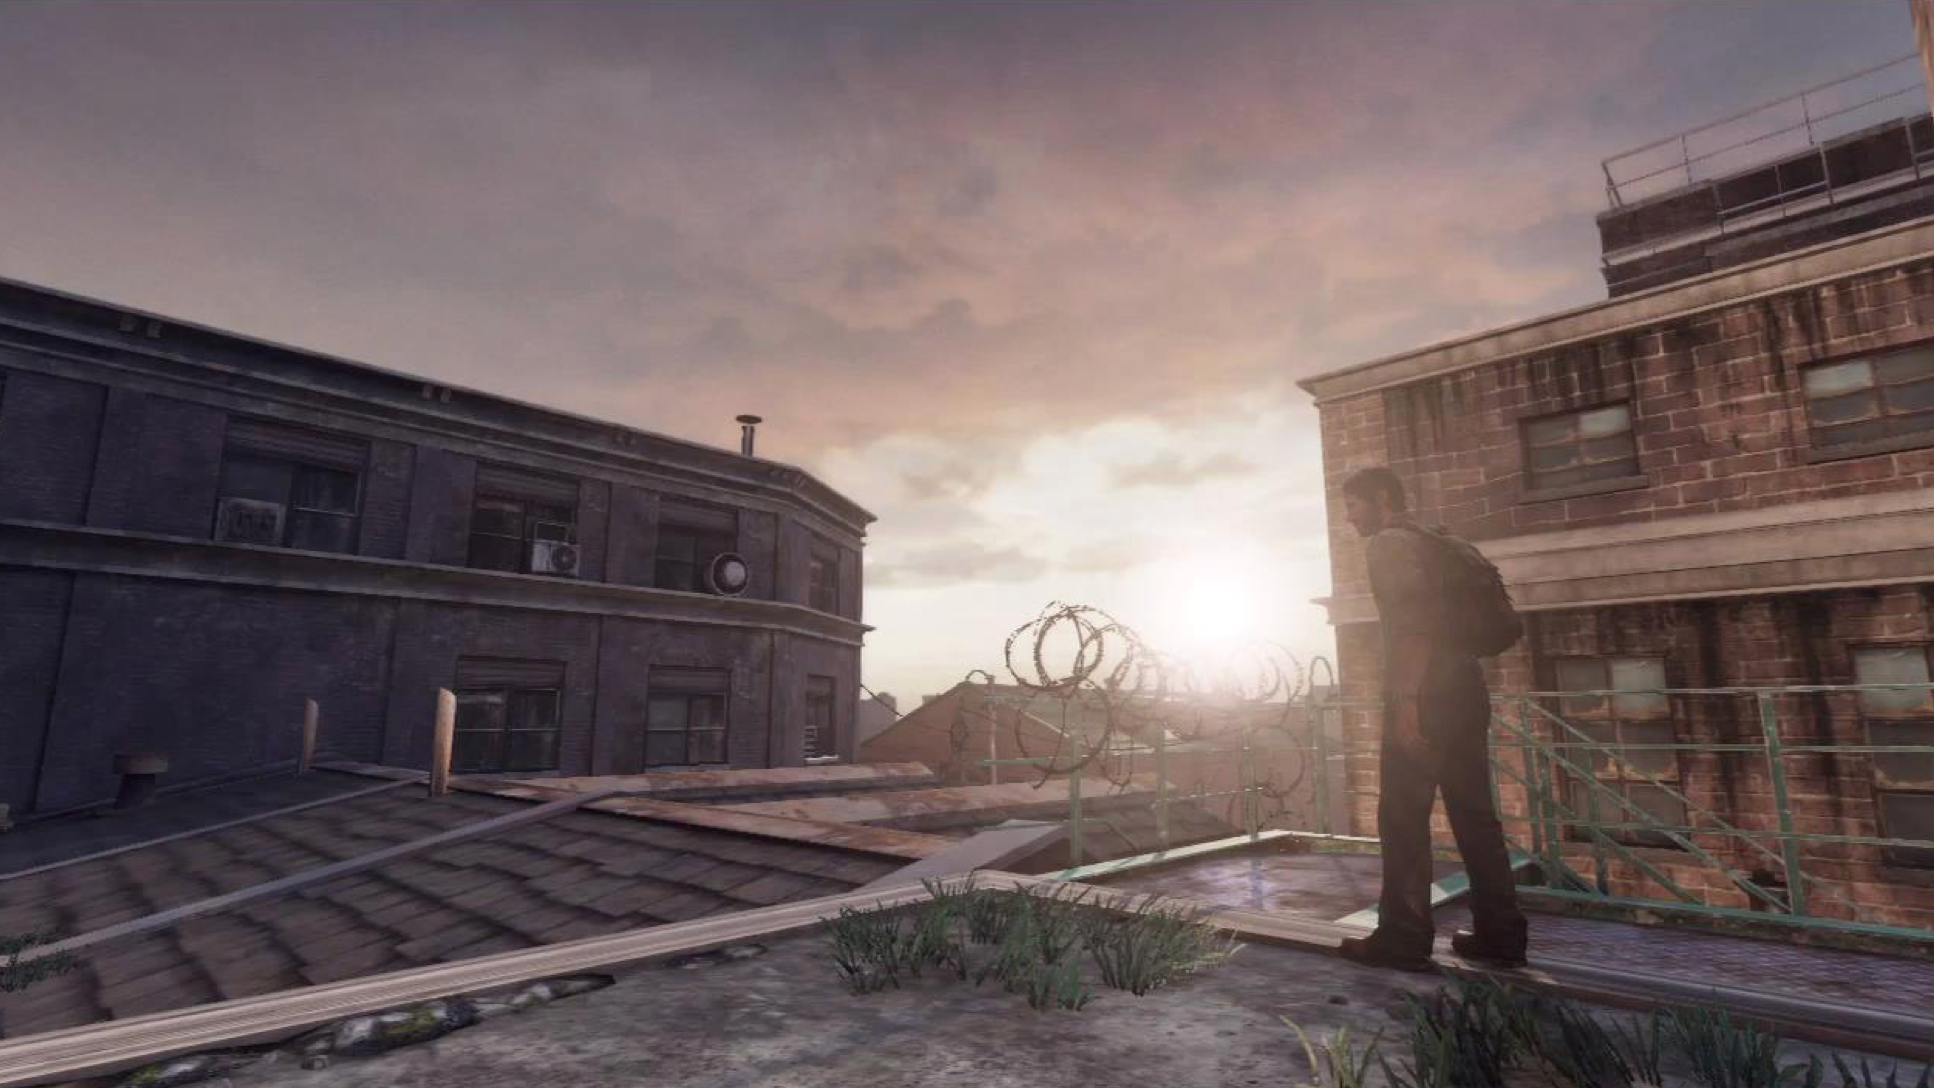
\includegraphics[scale=0.4]{img/result_cloud_sphere.png}
    \caption{Результат классического метода визуализации облаков}
    \label{img:result_sphere}
\end{figure}

При необходимости учета динамического освещения солнца можно генерировать облака при помощи частиц \cite{hpg.20141101}.

\begin{figure}[H]
    \centering
    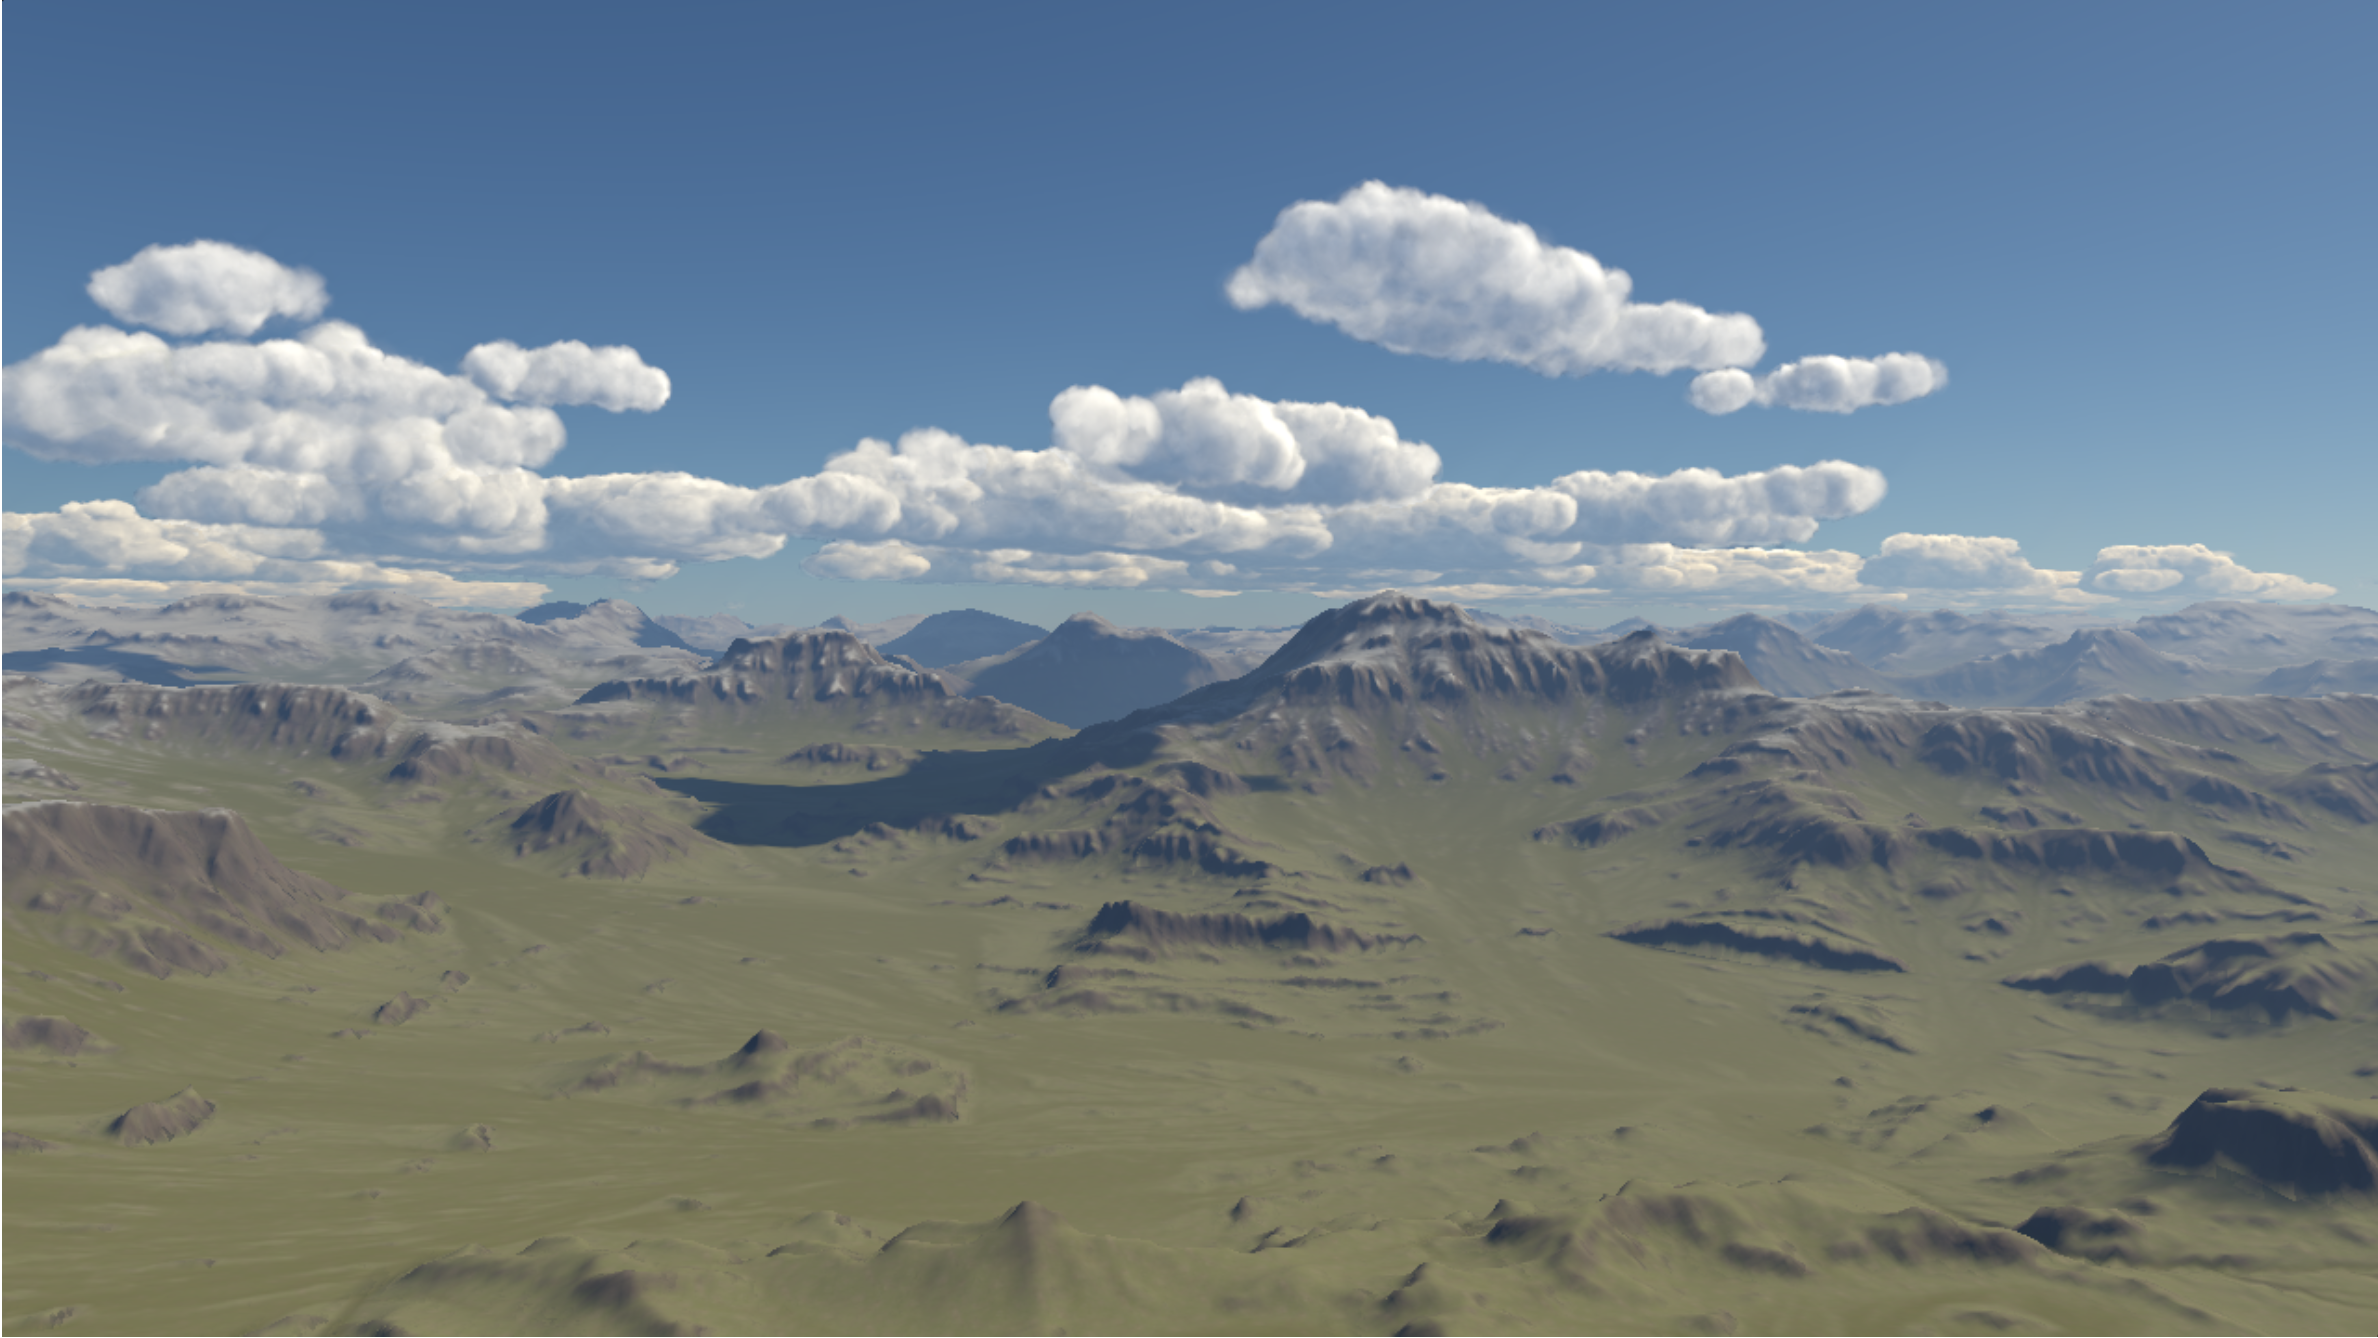
\includegraphics[scale=0.4]{img/ysov.png}
    \caption{Результат алгоритма частиц}
    \label{img:ysov}
\end{figure}

Третий метод называется алгоритм лучевого марша, являющий самым трудоемким из всех алгоритмов
визуализации облаков. Данный алгоритм позволяет визуализировать динамически освещенные
облака \cite{Sch16}. С помощью нескольких параметров этот метод позволяет строить сложные облачные
формы с высокой детализацией как видно на рисунке \ref{img:raymach}.

\begin{figure}[H]
    \centering
    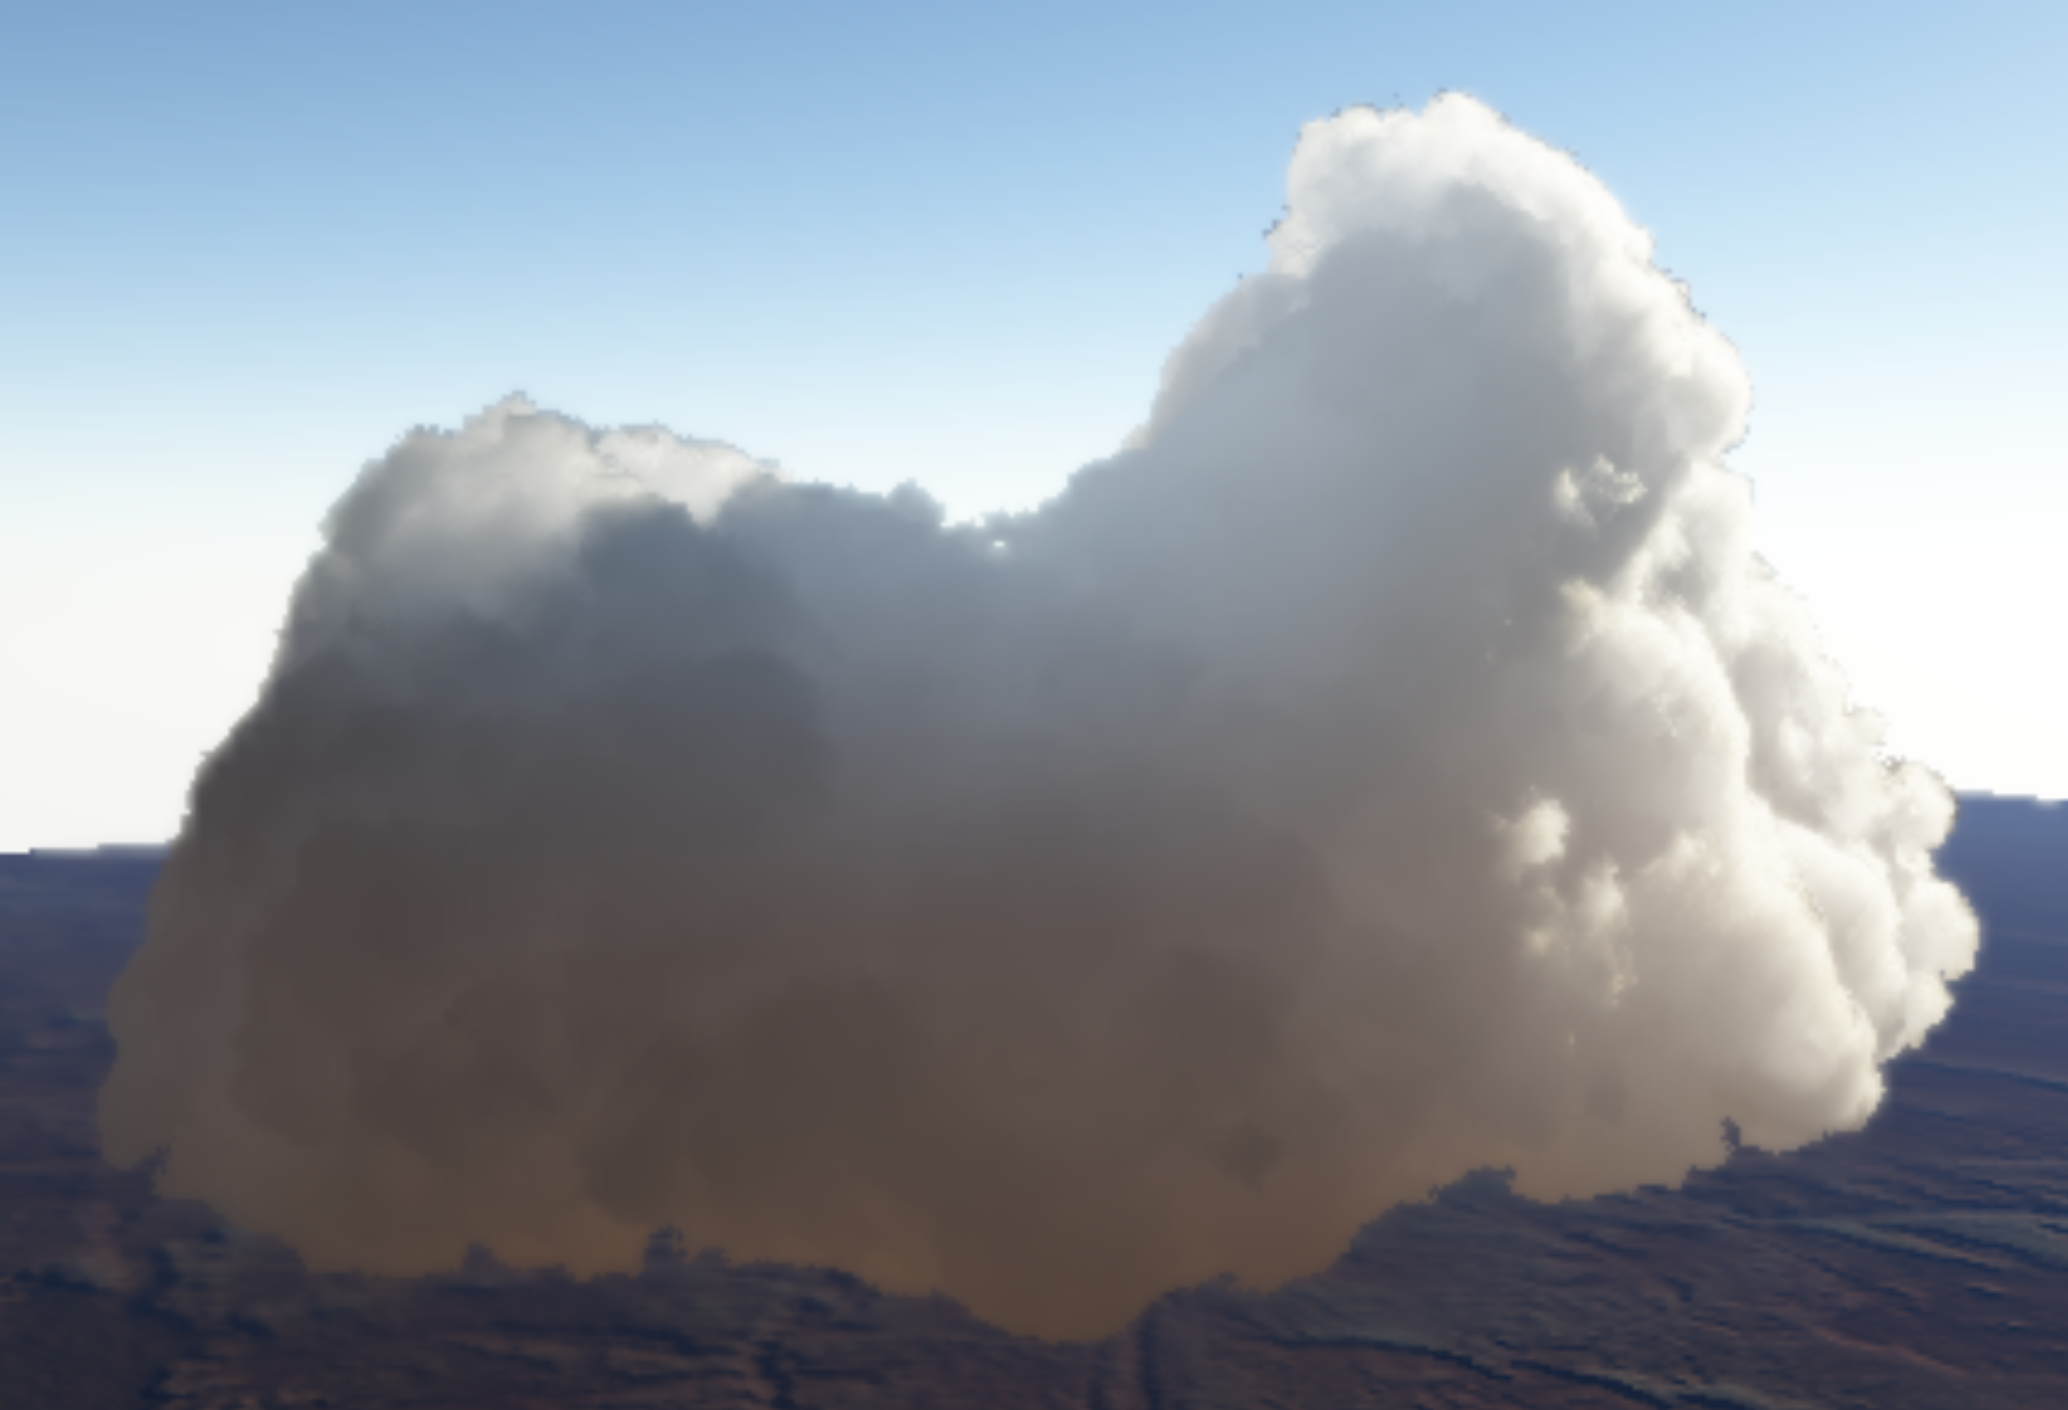
\includegraphics[scale=0.4]{img/raymach.png}
    \caption{Результат алгоритма лучевого марша}
    \label{img:raymach}
\end{figure}

\subsection{Градиентные шумы}

Для генерации форм и текстур облаков используются алгоритмы градиентных шумов.
Шум это беспорядочные колебания физической природы. В данной работе используется два алгоритма
генерации шумов: Перлина и Ворлей.

\subsubsection{Шум Перлина}

Шум перлина применяется для любого $n$-мерного пространства. Данный алгоритм состоит из трех этапов.

\begin{enumerate}
    \item Заполнение сетки псевдослучайными векторами
    \item Вычисление значения в каждой точке
    \item Интерполяция между этими точками
\end{enumerate}

Пространство делится $n$-мерной сеткой, которая заполняется псевдослучайными единичными векторами.
На рисунке \ref{img:vectors} представлен пример для 2-мерного пространства.

\begin{figure}[H]
    \centering
    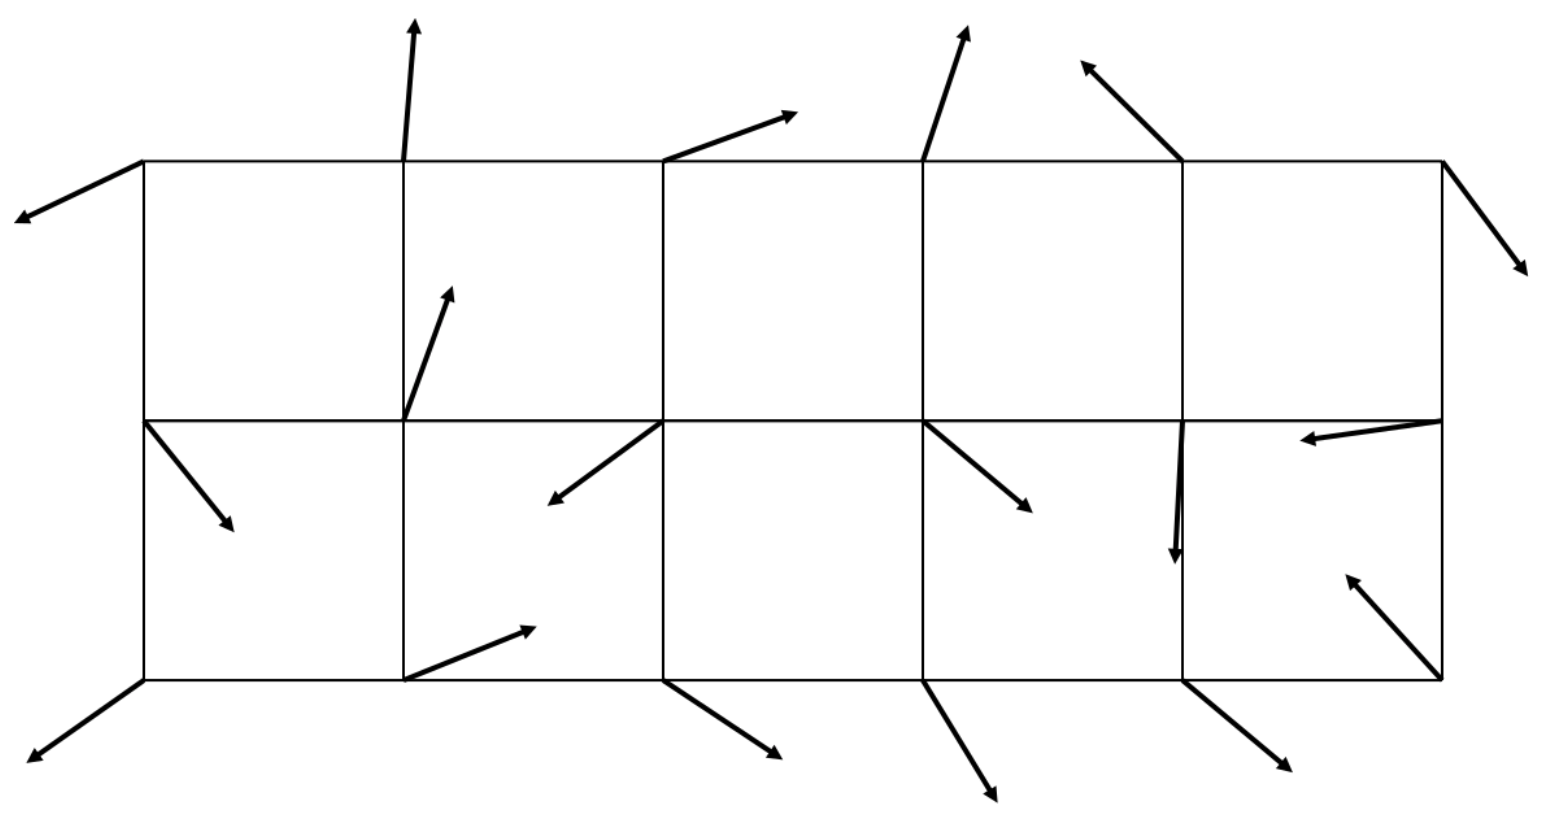
\includegraphics[scale=0.6]{img/vectors.png}
    \caption{Сетка псевдослучайных векторов}
    \label{img:vectors}
\end{figure}

После необходимо интерполировать значения внутри сетки. Делается это при помощи скалярного произведения векторов

\begin{figure}[H]
    \centering
    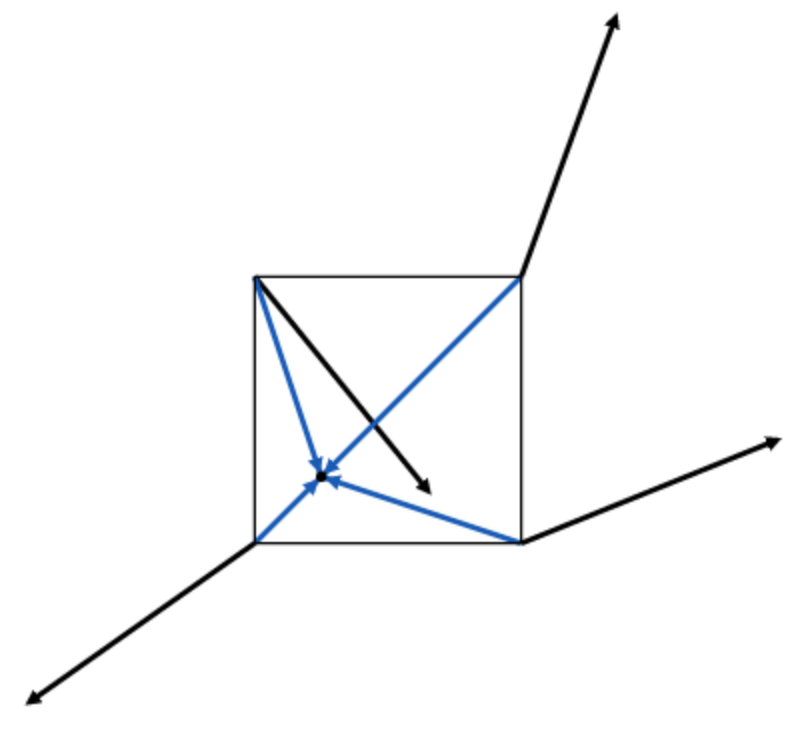
\includegraphics[scale=0.6]{img/interpolation.png}
    \caption{Интерполяция значений шума}
    \label{img:interpolation}
\end{figure}

\begin{figure}[H]
    \centering
    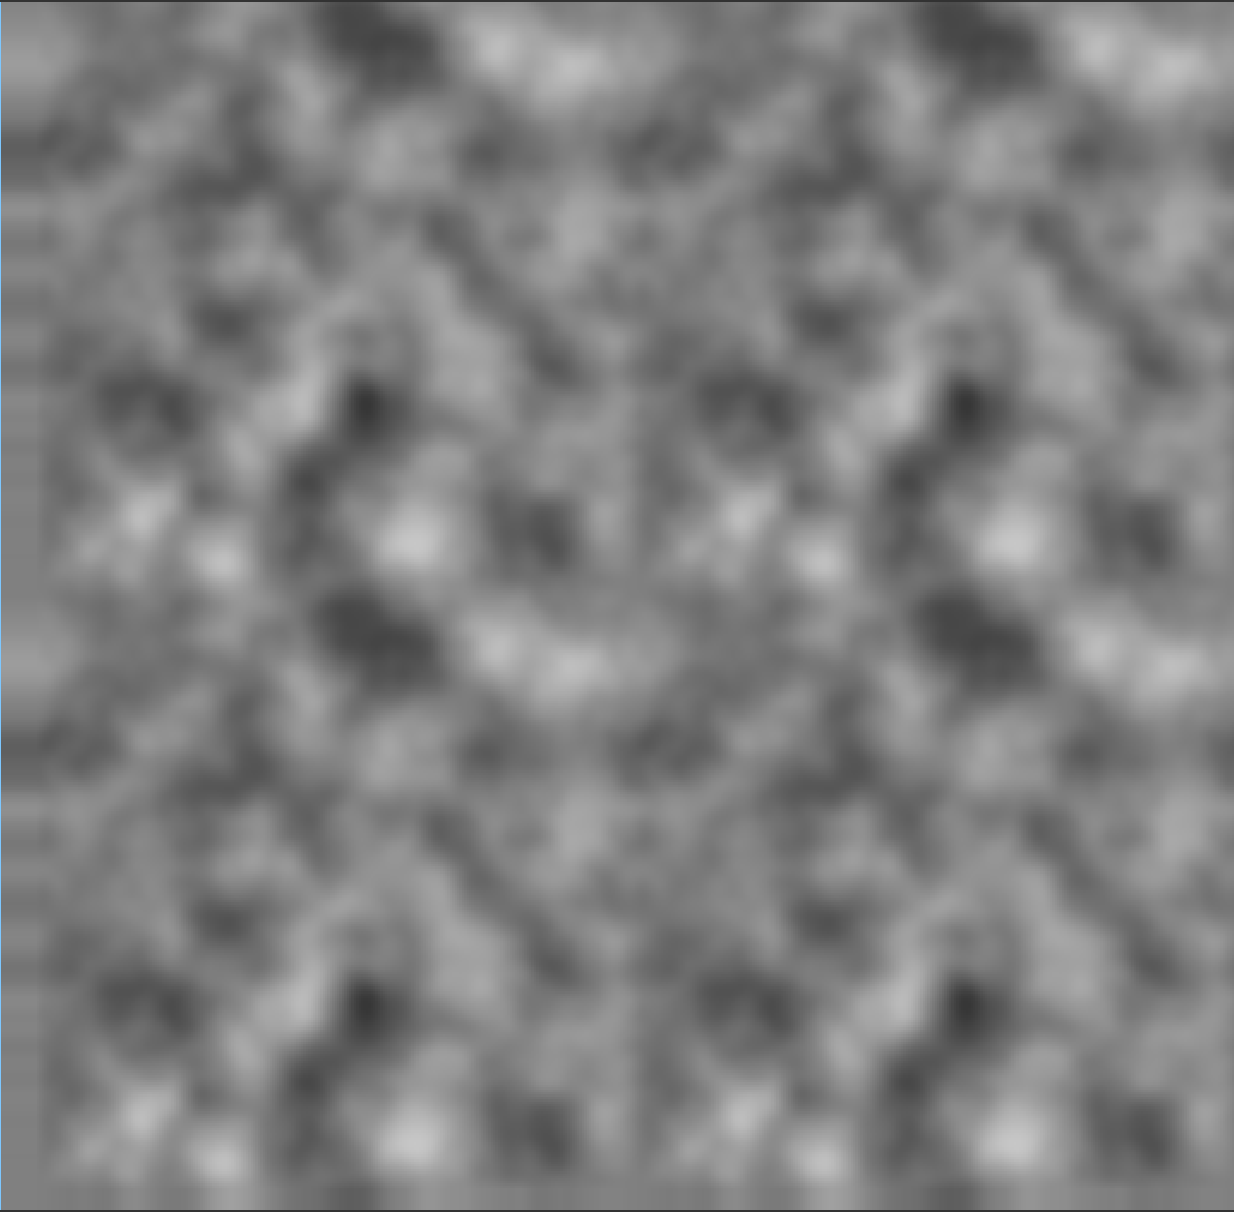
\includegraphics[scale=0.4]{img/perlin.png}
    \caption{Шум Перлина}
    \label{img:perlin}
\end{figure}

\subsubsection{Шум Ворлей}

\begin{figure}[H]
    \centering
    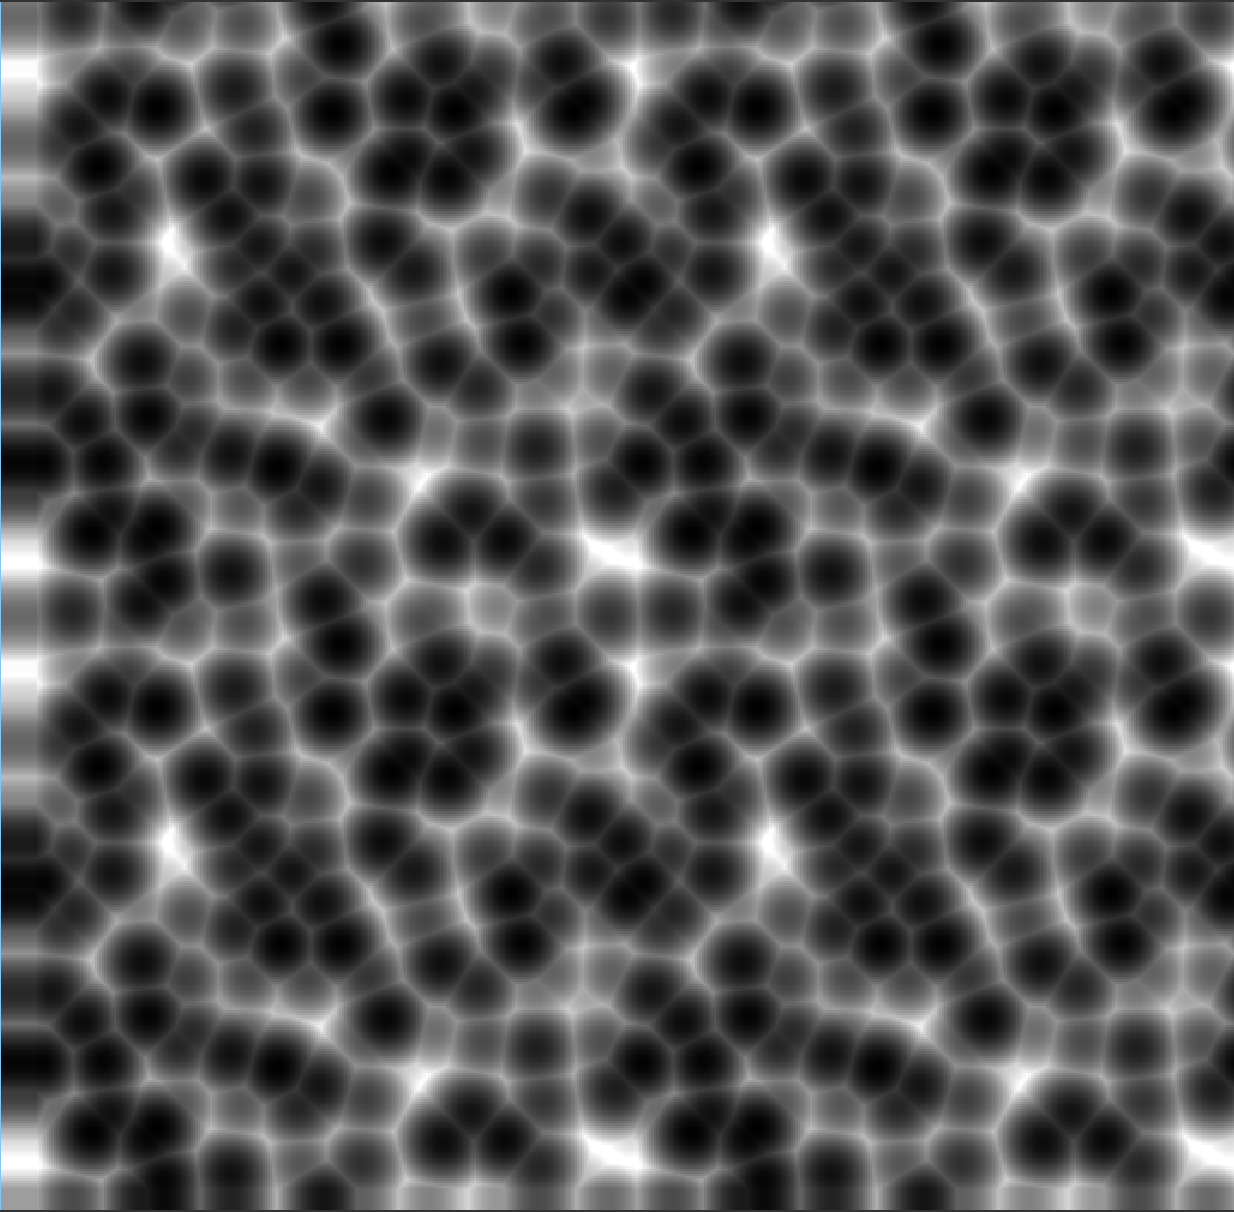
\includegraphics[scale=0.4]{img/worley.png}
    \caption{Шум Ворлея}
    \label{img:perlin}
\end{figure}

Если из максимального значения интенсивности вычесть значение шума Ворлей, можно получить результат как на рисунке \ref{img:worley2}

\begin{figure}[H]
    \centering
    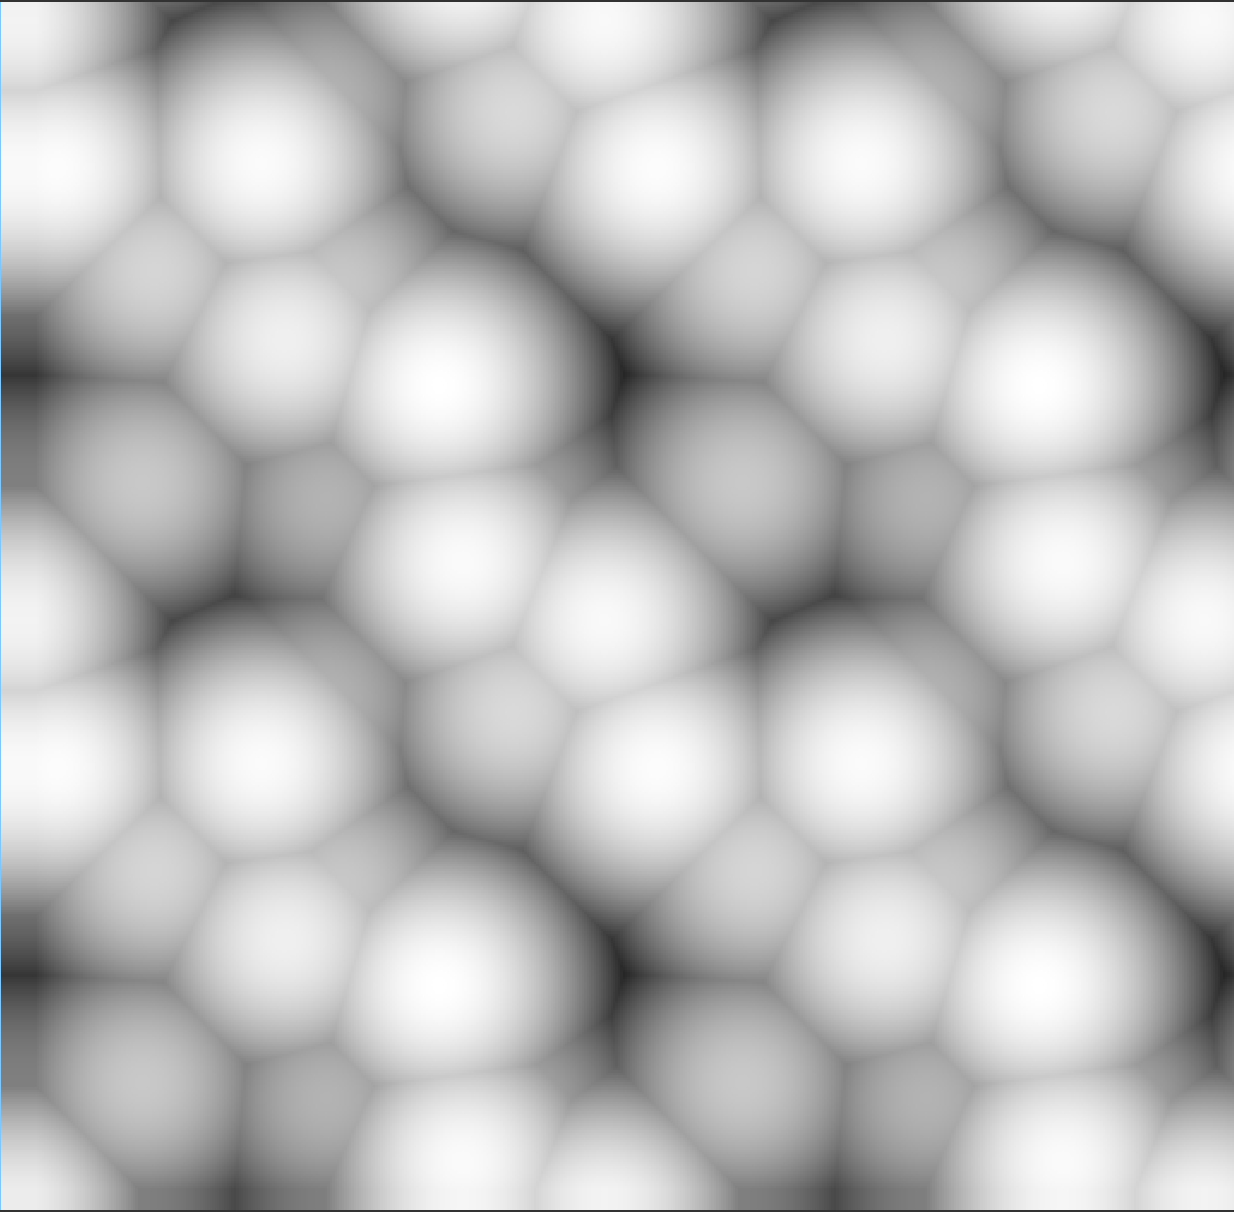
\includegraphics[scale=0.4]{img/worley2.png}
    \caption{Обратный шум Ворлея}
    \label{img:worley2}
\end{figure}

\begin{figure}[H]
    \centering
    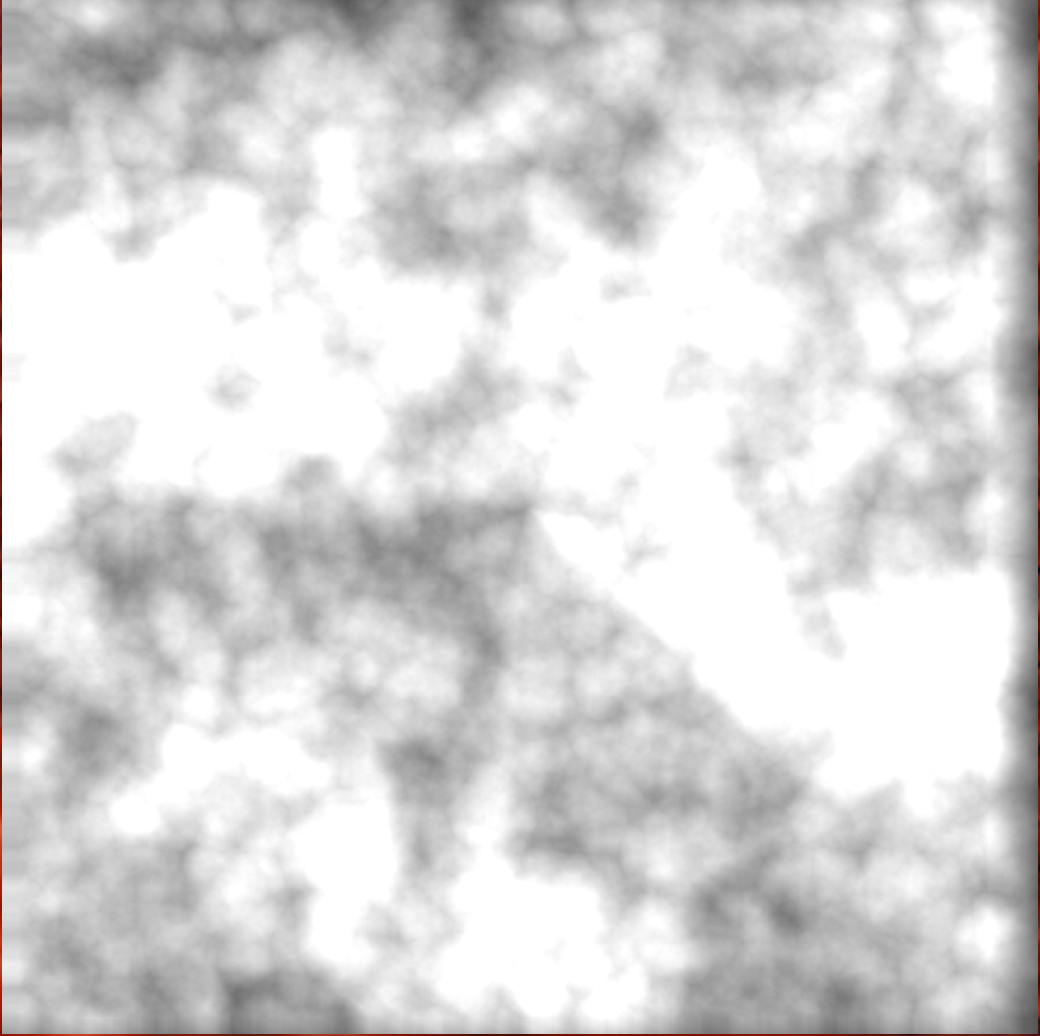
\includegraphics[scale=0.4]{img/result_noise.png}
    \caption{Результат объединения шумов}
    \label{img:result_noise}
\end{figure}

\subsection{Тени}

Реалистичное изображение не может быть без теней. Для реализации теней используется алгоритм, использующий
буфер глубины.

\subsection{Окружение}

Для создания окружающего пространства чаще всего используется куб с наложенными текстурами.

\section{Обзор и анализ существующих программных систем и обоснование необходимости разработки}
